\documentclass{article}
\usepackage{graphicx} % Required for inserting images
\usepackage[italian]{babel}
\usepackage[hidelinks]{hyperref}
\usepackage{algorithm}
\usepackage{algpseudocode}

\title{Reti di elaboratori}
\author{Leonardo Ganzaroli}
\date{}

\begin{document}

\maketitle

\addcontentsline{toc}{section}{\protect\numberline{}Introduzione}

\tableofcontents

\hypersetup{allcolors=black}

\newpage

\section*{Introduzione}

Questi appunti sono derivanti principalmente dalle slide del corso di \textit{Reti di elaboratori} che ho svolto durante la laurea Triennale di informatica all'università "La Sapienza".

\newpage

\section{Reti ed Internet}

\subsection{Internet}

\textbf{Definizione} Una rete è un'infrastruttura composta da \textit{nodi} collegati tramite \textit{link}.\newline

\noindent I nodi si possono dividere in 2 categorie:
\begin{enumerate}
    \item Terminali
        \begin{itemize}
            \item \textbf{Server}
            \item \textbf{Host}
        \end{itemize}
    \item Dispositivi di interconnessione
        \begin{itemize}
            \item \textbf{Router}

                Connette più reti.
            
            \item \textbf{Switch}

                Connette più terminali in una rete.
            
            \item \textbf{Modem}\newline
        \end{itemize}
\end{enumerate}

\noindent I link possono essere diversi:
\begin{itemize}
    \item Cavo coassiale
    \item Fibra ottica
    \item Doppino intrecciato
    \item Onde elettromagnetiche\newline
\end{itemize}

\noindent Le reti stesse si possono classificare in base alla loro dimensione:
\begin{itemize}
    \item \textbf{PAN} (Personal Area Network)
    \item \textbf{LAN} (Local $\ldots)$
    \item \textbf{MAN} (Metropolitan $\ldots)$
    \item \textbf{WAN} (Wide $\ldots)$
    \item \textbf{Internet}\newline
\end{itemize}

\begin{figure}[ht]
    \centering
    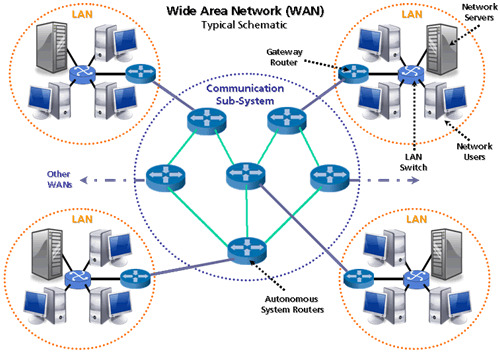
\includegraphics[width=0.7\linewidth]{wan.jpg}
    \caption{Esempio di rete}
    \label{fig:net}
\end{figure}

\newpage

\noindent\textbf{Definizione} Internet è la rete di tutte le reti.\newline

\noindent Si può dividere in 3 elementi:
\begin{enumerate}
    \item \textbf{Network Edge}

        L'insieme di tutti i nodi terminali connessi.

    \item \textbf{Access Network}

        I collegamenti tra i terminali e il primo Router.

    \item \textbf{Nucleo}

        La connessione tra le sottoreti.\newline
    
\end{enumerate}

\noindent Il nucleo stesso presenta una divisione a livelli, la connessione tra questi avviene tramite gli \textit{Internet Exchange Point}.\newline

\noindent L'accesso ad Internet può avvenire in diversi modi:
\begin{itemize}
    \item Via cavo
    \item Via DSL
    \item Via rete cellulare
    \item Via WLAN\newline
\end{itemize}

\subsection{Comunicazione}

\textbf{Definizione} Dividendo un messaggio da inviare in blocchi si ottengono i pacchetti.\newline

\noindent\textbf{Definizione} La commutazione è l'azione che sposta l'informazione in input ad un nodo all'output giusto, avviene in 2 modi:
\begin{enumerate}
    \item \textbf{Pacchetto}

        I singoli pacchetti arrivano al destinatario "rimbalzando" tra i nodi, ognuno potrebbe seguire un percorso diverso.
    
    \item \textbf{Circuito}

        Per far comunicare due terminali viene instaurato un percorso fisico che non può essere usato da nessun'altro fino alla sua "liberazione", si può effettuare una divisione in tempo/frequenza per permettere a più circuiti di usare un link contemporaneamente.\newline
    
\end{enumerate}

\noindent\textbf{Definizione} L'instradamento è la determinazione del percorso che un pacchetto deve seguire.\newline

\noindent\textbf{Definizione} La larghezza di banda è:
\begin{enumerate}
    \item La larghezza dell'intervallo di frequenze del mezzo trasmissivo
    \item Il numero di $bit/s$ che il mezzo può trasmettere\newline
\end{enumerate}

\noindent\textbf{Definizione} Il throughput è la quantità di $bit/s$ passanti per un nodo.\newline

\noindent\textbf{Definizione} Il tempo necessario per inviare un pacchetto tra 2 nodi è detto latenza, è composto da:
\begin{itemize}
    \item Lat. di trasmissione

        Tempo necessario per immetterlo sul link.

    \item Lat. di propagazione

        Tempo necessario per arrivare alla destinazione.

    \item Lat. di queueing

        Eventuale tempo passato in attesa nella coda di trasmissione.

    \item Lat. di elaborazione

        Tempo dovuto ad operazioni del nodo.\newline
    
\end{itemize}

\subsection{Protocolli}

\textbf{Definizione} Un protocollo è un insieme di regole.\newline

\noindent Per permettere la comunicazione vengono divisi i vari compiti in livelli indipendenti, ognuno con il suo protocollo. Così facendo si possono far comunicare sistemi diversi instaurando dei collegamenti logici tra i vari livelli.\newline

\begin{figure}[ht]
    \centering
    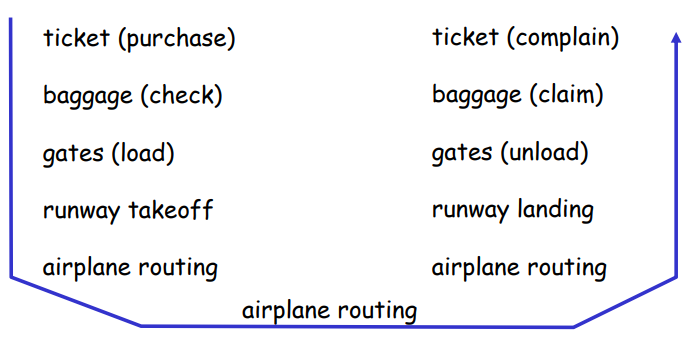
\includegraphics[width=0.6\linewidth]{stack.png}
    \caption{Esempio divisione a livelli}
    \label{fig:stack}
\end{figure}

\noindent I 2 modelli principali nell'ambito delle reti sono:

\begin{figure}[ht]
    \centering
    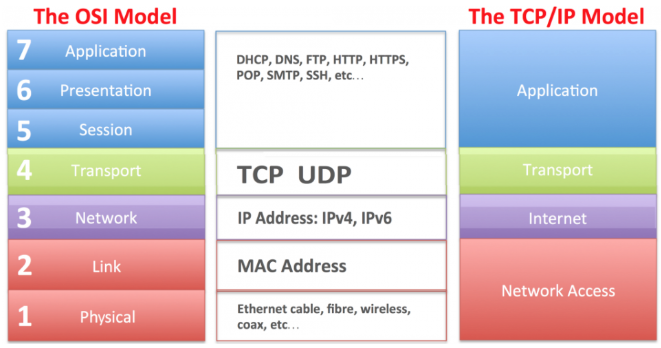
\includegraphics[width=0.8\linewidth]{models.png}
    \caption{ISO/OSI e TCP/IP}
    \label{fig:iso_tcp}
\end{figure}

\noindent Quando un messaggio deve essere inviato attraversa prima tutti i livelli partendo dall'alto, quando arriva al destinatario avviene il processo inverso.\newline

\noindent Ogni livello aggiunge un header con delle informazioni al messaggio prima di passarlo al livello inferiore (incapsulamento).\newline

\section{Livelli}

\subsection{Collegamento}

Fornisce i seguenti servizi:
\begin{itemize}
    \item Framing 
    \item Consegna tra nodi adiacenti
    \item Rilevamento e correzione errori
    \item Controllo del flusso
    \item Accesso al link\newline
\end{itemize}

\noindent Viene diviso in 2 sottolivelli:
\begin{enumerate}
    \item \textbf{LLC}
    \item \textbf{MAC}\newline
\end{enumerate}

\noindent\textbf{Definizione} L'indirizzo MAC è un indirizzo identificativo usato localmente, esso viene assegnato ad ogni scheda di rete ed è usato per inviare frame ad un'altra scheda fisicamente connessa.\newline

\begin{figure}[ht]
    \centering
    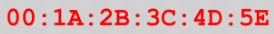
\includegraphics[width=0.5\linewidth]{mac.png}
    \caption{Indirizzo MAC}
    \label{fig:mac}
\end{figure}

\noindent Per trovare ed eventualmente risolvere errori ci sono diversi modi:
\begin{itemize}
    \item \textbf{Parity Checking}

    \item \textbf{Parity Checking multidimensionale}

    \item \textbf{CRC}\newline

\end{itemize}

\noindent Si individuano 2 tipi di collegamenti:
\begin{enumerate}
    \item \textbf{Punto-punto}
    \item \textbf{Broadcast}\newline
\end{enumerate}

\noindent Essendo diversi presentano un funzionamento che richiede protocolli specifici per effettuare correttamente trasmissioni di dati.\newline

\subsubsection{Protocolli}
\begin{itemize}
    \item \textbf{PPP}

        Usato per comunicazioni dirette tra due nodi.

    \item \textbf{ALOHA}
        \begin{itemize}
            \item \textbf{Slotted}
            
                Assumendo che i frame abbiano dimensioni uguali:
                    \begin{itemize}
                        \item Il tempo si divide in intervalli di lunghezza pari al tempo necessario per trasmettere un frame
                        \item I nodi sono sincronizzati
                        \item Quando arriva un frame aspetta il prossimo slot temporale per inviarlo
                        \item In caso di collisioni riprova la trasmissione nello slot successivo con una certa probabilità
                    \end{itemize}

            \item \textbf{Pure}

                Le uniche differenze con il precedente sono:
                    \begin{itemize}
                        \item Il tempo non viene diviso
                        \item Quando un frame arriva viene subito inviato
                    \end{itemize}

            \end{itemize}

        \item \textbf{CDMA}

        \item \textbf{TDMA}

        \item \textbf{FDMA}
                    
        \item \textbf{CSMA}

            Protocollo ad accesso casuale, a grandi linee:
                \begin{itemize}
                    \item Prima di trasmettere ascolta il canale
                    \item Se inattivo trasmetti, altrimenti aspetta
                \end{itemize}
            
                Ce ne sono di diversi tipi, 2 sono:
                    \begin{itemize}
                        \item \textbf{CD}

                            In caso di collisione il nodo trasmittente interrompe la trasmissione ed invia un apposito segnale per indicarla, poi torna in attesa.

                        \item \textbf{CA}

                            \begin{itemize}
                                \item Non c'è rilevamento delle collisioni
                                \item Si usa un ACK per capire se la trasmissione è riuscita
                                \item C'è un ascolto anche per il messaggio ACK
                                \item La collisione può avvenire anche per gli ACK
                            \end{itemize}
                        
                    \end{itemize}

        \item \textbf{ARP}

            Permette di associare un indirizzo MAC ad un indirizzo IP, ogni nodo possiede una tabella che contiene le associazioni.
    
\end{itemize}


\subsection{Rete}

Lo scopo di questo livello è di effettuare l'inoltro e l'instradamento dei pacchetti, garantisce quindi una comunicazione logica tra sorgente e destinatario.\newline

\noindent Un fatto fondamentale è che ci si basa su un modello \textit{best effort}, ossia la consegna dei pacchetti, il tempo necessario, etc$\ldots$ non è garantita.\newline

\subsubsection{IP}

\noindent Il protocollo usato a questo livello è l'IP, esso è formato da:
\begin{itemize}
    \item \textbf{Interfaccia}

        Collegamento alla rete fisica.

    \item \textbf{Sottorete}

        L'insieme di interfacce direttamente raggiungibili.

    \item \textbf{Indirizzo IP}

        Un indentificatore associato ad un'interfaccia.\newline
    
\end{itemize}

\begin{figure}[ht]
    \centering
    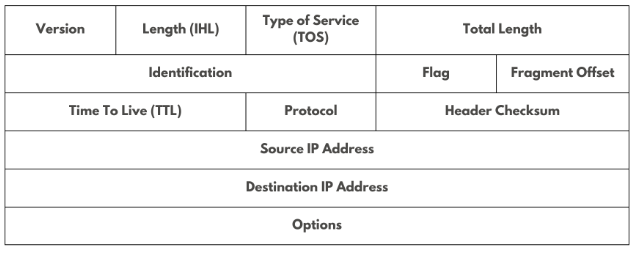
\includegraphics[width=0.8\linewidth]{ip.png}
    \caption{Header IP}
    \label{fig:h_ip}
\end{figure}

\noindent Ci sono 2 versioni dell'indirizzo IP:
\begin{enumerate}
    \item \textbf{IPv4}

        32 bit divisi in quattro gruppi.
    
    \item \textbf{IPv6}

        128 bit divisi in 8 gruppi di 2 byte.\newline
    
\end{enumerate}

\noindent Dato che il passaggio a IPv6 ancora non è completo si usa il \textit{NAT} per risparmiare indirizzi, ossia il Router associa un unico indirizzo IP esterno a tutti i dispositivi della rete interna.\newline 

\subsubsection{Router}

I Router sono i dispositivi principali nel caso la comunicazione non sia interna alla sottorete, mantengono delle tabelle contenenti le varie destinazioni di una certa rete ed eventualmente la sua "distanza".\newline

\noindent La struttura generale è la seguente:
\begin{itemize}
    \item Porte Input/Output connesse ai link

        Composte da:
        \begin{itemize}
            \item Memoria interna
            \item Terminazione di linea
            \item Interfaccia con livello inferiore
        \end{itemize}
        
    \item Struttura di commutazione tra le porte
    \item Processore di instradamento\newline
\end{itemize}

\noindent In alcuni casi si potrebbe verificare un accodamento nelle porte che può portare ad una perdita di pacchetti, per minimizzare il problema si usano degli algoritmi di scheduling:
\begin{itemize}
    \item \textbf{FCFS}
    \item \textbf{Con priorità}
    \item \textbf{Round Robin}
    \item \textbf{WFQ}\newline
\end{itemize}

\noindent Alcuni collegamenti possono avere una dimensione di trasferimento massima sul link, in questo caso avviene la frammentazione del pacchetto con successiva ricostruzione da parte del destinatario.\newline

\noindent Per effettuare lo spostamento verso l'output ci sono 3 modi:

\begin{figure}[ht]
    \centering
    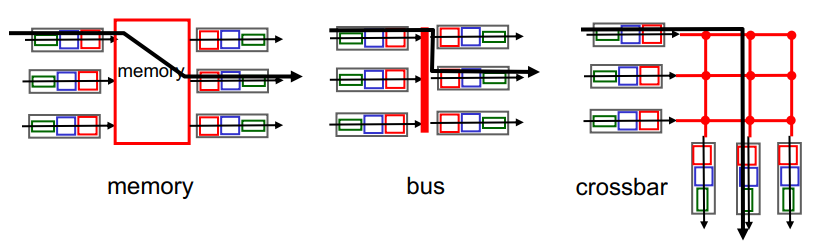
\includegraphics[width=0.9\linewidth]{swfa.png}
    \label{fig:sw_fa}
\end{figure}

\subsubsection{Algoritmi di instradamento}

Gli algoritmi di routing vengono classificati in:
\begin{itemize}
    \item Statici/Dinamici
    \item Globali/Decentralizzati\newline
\end{itemize}

\noindent Notazione:
\begin{itemize}
    \item $c_{x,y}$ è il costo del link tra i nodi $x$ e $y$
    \item $D(v)$ è la stima del costo dalla sorgente a $v$
    \item $p(v)$ è il nodo predecessore\newline
\end{itemize}

\noindent Considerando la sua struttura è possibile rappresentare una rete come un grafo, di conseguenza si può usare una variante dell'algoritmo di Dijkstra:

\begin{algorithm}[ht]
\begin{algorithmic}
\State Link-State(G,x):

\State $R=\{x\}$

\For{$v\in V(G)$}

    \If{$\exists(u,v)\in E(G)$}

        \State $D(v)=c_{u,v}$

    \Else

        \State $D(v)=\infty$

    \EndIf

\EndFor

\While{$R\neq V(G)$}

    \State $w=min_{w\in V(G)\setminus R}(D(w))$

    \State $R.add(w)$

    \For{$x\in V(G)\setminus R$}

        \If{$\exists(w,x)\in E(G)$}

            \State $D(x)=min(D(x),D(w)+c_{w,x})$

            \State $p(x)=w$

        \EndIf

    \EndFor

\EndWhile

\end{algorithmic}
\end{algorithm}

\noindent Un'altra possibilità è l'algoritmo Distance-vector, è basato sull'equazione di Bellman-Ford $D_x(y)=min_{v\in V(G)}(c_{x,v}+D_v(y))$. Si può riassumere in:
\begin{enumerate}
    \item Inizializza la tabella delle distanze
    \item Attendi un cambio di costo
    \item Ricalcola
    \item Invia le eventuali modifiche ai vicini
\end{enumerate}

\subsubsection{Protocolli}

\begin{itemize}
    \item \textbf{DHCP}

        Permette di assegnare dinamicamente indirizzi IP.

    \item \textbf{ICMP}

        Usato per scambiare messaggi a questo livello.

    \item \textbf{RIP}

        Instradamento tramite Distance-vector.

    \item \textbf{OSPF}

        Instradamento tramite Link-State.

    \item \textbf{BGP}

        Instradamento tramite Path-vector.

    \item \textbf{IGMP}

        Usato per richiedere l'adesione ad un gruppo multicast.
    
\end{itemize}

\subsection{Trasporto}

Lo scopo di questo livello è di instaurare una connessione logica tra i processi applicativi in esecuzione sui dispositivi.\newline

\noindent Per identificare i processi viene fatto uso di un numero di porta ad essi associato, nell'Header inserito qui + Header IP saranno generalmente presenti:
\begin{itemize}
    \item IP + porta origine
    \item IP + porta destinatario
\end{itemize}

\begin{figure}[ht]
    \centering
    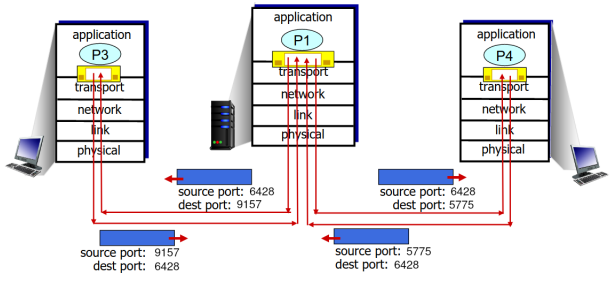
\includegraphics[width=0.9\linewidth]{transp.png}
    \caption{Esempio di comunicazione}
    \label{fig:transo}
\end{figure}

\subsubsection{UDP}

Il protocollo UDP è senza connessione e \textit{barebone}, quindi le informazioni inviate potrebbero arrivare in qualsiasi ordine o non arrivare proprio.\newline

\noindent Le sue caratteristiche lo rendono utile per i seguenti motivi:
\begin{itemize}
    \item Comunicazione veloce
    \item Dimensione minima dell'Header
    \item "Ignora" la congestione
    \item Presenta comunque un minimo controllo degli errori tramite Checksum\newline
\end{itemize}

\begin{figure}[ht]
    \centering
    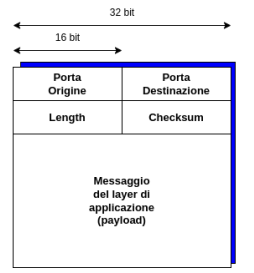
\includegraphics[width=0.35\linewidth]{head_udp.png}
    \caption{Header UDP}
    \label{fig:head_udp}
\end{figure}

\noindent Il checksum è essenzialmente la somma in complemento ad uno (con wraparound) degli altri campi.\newline

\noindent Per i motivi visti UDP viene usato dalle applicazioni che tollerano perdita di dati ma sono dipendenti dal tempo, per esempio il traffico audio/video (anche in tempo reale) è un candidato perfetto.\newline

\newpage

\subsubsection{TCP}

Questo protocollo invece è orientato alla connessione e la inizializza tramite \textit{handshaking} (a 3 vie), offre inoltre uno stream di byte affidabile ed ordinato.\newline

\begin{figure}[ht]
    \centering
    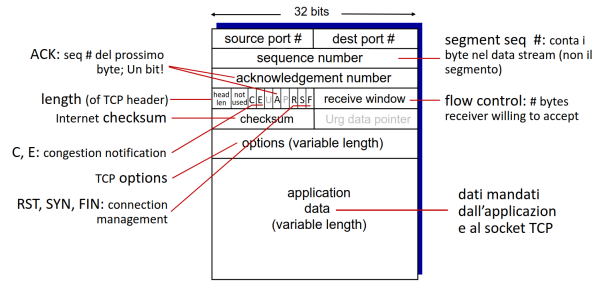
\includegraphics[width=0.85\linewidth]{head_tcp.png}
    \caption{Header TCP}
    \label{fig:head_tcp}
\end{figure}

\noindent Per garantire il trasporto usa:
\begin{itemize}
    \item \textbf{ACK cumulativi}
    \item \textbf{Numero di sequenza}

        Corrisponde al numero di sequenza del primo byte del settore data, invece per gli ACK è il byte successivo aspettato.
    
    \item \textbf{Timer}

        Fa riferimento al pacchetto più vecchio non confermato, se scade viene rinviato e si resetta.\newline
    
\end{itemize}

\noindent\textbf{Definizione} L'RTT è il tempo impiegato da un piccolo pacchetto per effettuare il percorso client$\rightarrow$server$\rightarrow$client.\newline

\noindent Questo protocollo gestisce inoltre sia il flusso (tramite la receive window) che la congestione con diversi metodi:
\begin{itemize}
    \item \textbf{Fast recovery}

        Si dimezza il rate di invio in caso di perdite rilevate.
    
    \item \textbf{Slow start}

        Partendo da un valore prefissato all'inizio della connessione, ogni RTT si raddoppia il numero di byte inviati fino alla prima perdita.\newline

\end{itemize}

\noindent

\begin{figure}[ht]
    \centering
    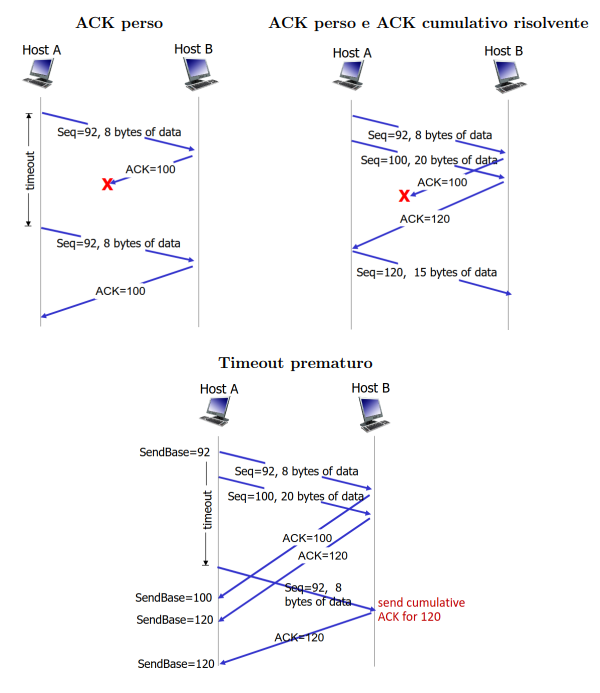
\includegraphics[width=0.8\linewidth]{ack.png}
    \caption{Alcuni casi}
    \label{fig:ack}
\end{figure}

\subsection{Applicazione}

\textbf{Definizione} Un paradigma di comunicazione è un metodo di scambio informazioni, i 2 più usati sono:
\begin{enumerate}
    \item \textbf{Client-Server}
    \item \textbf{P2P} \newline
\end{enumerate}

\noindent\textbf{Definizione} Un socket è un'astrazione software che permette ad un processo di inviare e ricevere messaggi a/da il socket di un altro processo.\newline

\noindent\textbf{Definizione} Un protocollo è stateless se non conserva informazioni sulle sessioni preceddenti.\newline

\subsubsection{HTTP}
\begin{itemize}
    \item Porta 80
    \item TCP
    \item Stateless
    \item Client-Server\newline
\end{itemize}

\noindent Le connessioni di questo tipo originariamente erano non persistenti, dalla versione 1.1 si possono creare anche connessioni persistenti.\newline

\noindent I messaggi vengono formattati in Ascii, la struttura di un messaggio è:
\begin{itemize}
    \item \textbf{Richiesta}
        \begin{itemize}
            \item Riga di richiesta
            \item Header
            \item Body
        \end{itemize}
    
    \item \textbf{Risposta}
        \begin{itemize}
            \item Riga di stato
            \item Header
            \item Body\newline
        \end{itemize}
\end{itemize}

\begin{figure}[ht]
    \centering
    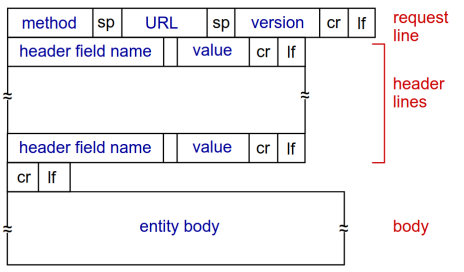
\includegraphics[width=0.7\linewidth]{http.png}
    \caption{Struttura richiesta}
    \label{fig:http}
\end{figure}

\newpage

\noindent I possibili metodi usati nella riga di richiesta sono:
\begin{itemize}
    \item \textbf{GET}

        Invio dati al server, presenti nell'URL.
    
    \item \textbf{POST}

        Invio dati al server, presenti nel Body.
    
    \item \textbf{HEAD}

        Richiesta esclusiva dell'Header che si riceverebbe usando GET.
    
    \item \textbf{PUT}

        Caricamento/Sostituzione file, non più usato.\newline
    
\end{itemize}

\noindent I possibili codici presenti nella riga di stato sono:
\begin{itemize}
    \item \textbf{1xx}

        Risposta contiene solo informazioni.
    
    \item \textbf{2xx}

        Richiesta andata a buon fine.
    
    \item \textbf{3xx}

        Avvenuto un reindirizzamento.
    
    \item \textbf{4xx}

        Errore nella richiesta.
    
    \item \textbf{5xx}

        Errore del server.\newline
    
\end{itemize}

\noindent\textbf{Definizione} Un cookie è un file di testo contenente informazioni, viene salvato nel client da parte del server.\newline

\noindent\textbf{Definizione} Un server proxy è un intermediario tra client e server.\newline

\newpage

\subsubsection{Posta elettronica}

\textbf{Definizione} Uno User Agent (UA) è un processo attivo sul client che informa l'utente di nuove e-mail ricevute, permette anche la lettura/scrittura di mail che vengono inviate poi all'MTA.\newline

\noindent\textbf{Definizione} Un Mail Transfer Agent (MTA) è un processo attivo sul server che invia e-mail ad un altro MTA.\newline

\noindent\textbf{Definizione} Un Mail Access Agent (MAA) è un processo attivo sul server che permette di leggere la posta in arrivo.\newline

\paragraph{SMTP}
\begin{itemize}
    \item Porta 25
    \item Ascii
    \item Interazione comando-risposta
    \item Invio diretto tra MTA\newline
\end{itemize}

\paragraph{MIME} $\ $\newline

\noindent Un protocollo avanzato che permette di usare messaggi multimediali.\newline

\paragraph{POP3}
\begin{itemize}
    \item Porta 110
    \item Stateless
    \item Scarica le mail dal server (vengono cancellate sul server)\newline
\end{itemize}

\paragraph{IMAP}
\begin{itemize}
    \item Porta 143
    \item Stateful
    \item Come POP3 ma le mail non vengono cancellate
\end{itemize}


\subsubsection{DNS}

\textbf{Definizione} Il Domain Name System viene usato per mappare i nodi della rete ad un nome identificativo, alcune delle sue funzioni sono:
\begin{itemize}
    \item Traduzione nome in IP
    \item Distribuzione del carico
    \item Host Aliasing\newline
\end{itemize}

\noindent Essendo un sistema decentralizzato presenta una gerarchia a livelli:
\begin{enumerate}
    \item \textbf{Root}
    \item \textbf{TLD}
    \item \textbf{Server autoritativi}
    \item \textbf{Server locali}\newline
\end{enumerate}

\noindent Il protocollo omonimo:
\begin{itemize}
    \item Porta 53
    \item UDP
    \item Stateless\newline
\end{itemize}

\noindent Richieste e risposte hanno la stessa struttura:

\begin{figure}[ht]
    \centering
    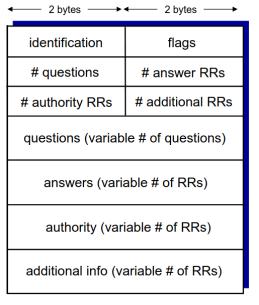
\includegraphics[width=0.35\linewidth]{dns.png}
    \label{fig:dns}
\end{figure}

\newpage

\subsubsection{FTP}
\begin{itemize}
    \item Porta 20 (dati)
    \item Porta 21 (controllo)
    \item 2 connessioni TCP
    \item Stateful\newline
\end{itemize}

\noindent Permette di scambiare file tra client e server.\newline

\subsubsection{BitTorrent}
\begin{itemize}
    \item Solitamente porte [6881-6889]
    \item TCP
    \item P2P\newline
\end{itemize}

\noindent\textbf{Definizione} Un torrent è un insieme di peer che si scambiano pezzi di file.\newline

\noindent\textbf{Definizione} Un tracker è un dispositivo che tiene traccia dei peer in un torrent.\newline

\noindent Durante il download un peer svolge anche la funzione di uploader.\newline

\end{document}
